\documentclass[journal]{IEEEtran}

\usepackage{siunitx}

\ifCLASSINFOpdf
  \usepackage[pdftex]{graphicx}

\else
\fi

\usepackage{listings}
\usepackage{xcolor}
\usepackage{tabularx}
\usepackage{booktabs}
\usepackage{tikz}

\usetikzlibrary{arrows.meta,positioning}

\definecolor{codegreen}{rgb}{0,0.6,0}
\definecolor{codegray}{rgb}{0.5,0.5,0.5}
\definecolor{codepurple}{rgb}{0.58,0,0.82}
\definecolor{backcolour}{rgb}{0.95,0.95,0.92}

\lstdefinestyle{mystyle}{
    backgroundcolor=\color{backcolour},   
    commentstyle=\color{codegreen},
    keywordstyle=\color{magenta},
    numberstyle=\tiny\color{codegray},
    stringstyle=\color{codepurple},
    basicstyle=\ttfamily\footnotesize,
    breakatwhitespace=false,         
    breaklines=true,                 
    captionpos=b,                    
    keepspaces=true,                 
    numbers=left,                    
    numbersep=5pt,                  
    showspaces=false,                
    showstringspaces=false,
    showtabs=false,                  
    tabsize=2
}

\lstset{style=mystyle}

\usepackage{hyperref}
\hypersetup{
    colorlinks=true,
    linkcolor=blue,
    citecolor=blue,      
    urlcolor=blue,
    pdftitle={Proyecto Final IoT - Arenero inteligente con acceso selectivo - Grupo 4},
    pdfpagemode=FullScreen,
    }

\urlstyle{same}

\hyphenation{op-tical net-works semi-conduc-tor}

\begin{document}

\title{Proyecto Final IoT - Grupo 4}

\author{Luis Izaguirre, Harold Canto, Joel Jimenez, y Hans Mendoza}

\maketitle

\IEEEpeerreviewmaketitle



\section{Introducción}

En hogares donde conviven varios gatos, la gestión de los recursos individuales (especialmente los areneros) se vuelve un reto tanto higiénico como de bienestar animal. Compartir un mismo arenero puede incrementar el estrés, dificultar el control de la salud de cada gato y generar conflictos de territorialidad. Aunque existen areneros automáticos en el mercado, la mayoría se centra en la autolimpieza o el monitoreo básico, sin resolver el problema de controlar qué gato accede a cada arenero.

En este contexto, el uso de tecnologías de Internet de las Cosas (IoT) permite diseñar soluciones que integran identificación inalámbrica, control embebido y mecanismos de acceso físico. El proyecto propone un arenero inteligente con acceso selectivo, donde solo un gato autorizado puede ingresar mediante un collar con tecnología Bluetooth Low Energy (BLE) y una compuerta motorizada controlada por un microcontrolador de bajo costo.

\subsection{Problemática}

El problema técnico a resolver consiste en diseñar e implementar un sistema capaz de:
\begin{itemize}
    \item Identificar de forma fiable a un gato específico mediante un collar BLE.
    \item Detectar su proximidad al arenero a partir de la intensidad de la señal (RSSI).
    \item Accionar una compuerta motorizada que se abra únicamente ante la detección del gato autorizado y se cierre de manera segura.
\end{itemize}

De este modo, se busca evitar que otros gatos utilicen el arenero, mejorar el control individual de higiene y uso, y explorar una arquitectura IoT reproducible que combine identificación inalámbrica, electrónica embebida y actuadores en un entorno doméstico real.

\subsection{Marco Teórico}

Para el desarrollo del arenero inteligente con acceso selectivo se consideran los siguientes conceptos clave:

\begin{itemize}
    \item \textbf{Internet de las Cosas (IoT):} Paradigma en el que dispositivos físicos incorporan sensores, actuadores, procesamiento embebido y conectividad para ofrecer servicios automatizados. En este proyecto, el arenero se concibe como un nodo IoT que percibe (detección de collar y presencia), decide (lógica de control) y actúa (apertura/cierre de compuerta).

    \item \textbf{Arquitectura IoT en capas:} Capa de percepción (sensores, servomotor), capa de red (BLE y WiFi) y capa de aplicación (registro y posible visualización de eventos). Esta estructura guía el diseño de la electrónica y del firmware, alineado con el objetivo de integrar identificación inalámbrica, control embebido y posibles servicios remotos.

    \item \textbf{Bluetooth Low Energy (BLE) y RSSI:} BLE es una tecnología de comunicación de corto alcance y bajo consumo, adecuada para \emph{beacons} en collares de animales \cite{walker2024ble,farine2024blebeacons}. El indicador de intensidad de señal recibida (RSSI) permite estimar proximidad de forma aproximada, lo que se aprovecha para decidir cuándo abrir la compuerta sólo si el gato autorizado está lo suficientemente cerca.

    \item \textbf{Sistemas \emph{wearables} para animales:} Dispositivos electrónicos montados en collares o arneses que registran actividad o comportamiento \cite{fonseca2023wearable}. Aportan criterios sobre peso máximo, fijación, autonomía y robustez, directamente vinculados al objetivo de diseñar un collar BLE cómodo y estable para el gato.

    \item \textbf{Identificación electrónica: RFID y BLE:} RFID asigna un identificador único a cada individuo mediante tags leídos a corta distancia, mientras que BLE emplea \emph{beacons} activos. Estudios comparativos analizan coste, consumo y precisión de ambas tecnologías en escenarios indoor \cite{gendy2023blevsrfid}, lo que respalda la elección de BLE frente a RFID para cumplir el objetivo de identificación fiable con hardware de bajo costo y ESP32.

    \item \textbf{Control de acceso selectivo y actuadores:} Dispositivos que abren o bloquean el acceso a recursos (comida, refugio, arenero) utilizando la identidad detectada y actuadores como servomotores \cite{wild2023selective,brian2023petfeeder}. Este concepto sustenta el objetivo de accionar una compuerta motorizada que sólo se abra ante la detección del gato autorizado.

    \item \textbf{Areneros inteligentes y sensores de higiene:} Prototipos que integran microcontroladores (por ejemplo, ESP32/ESP8266), sensores de presencia o nivel de llenado y mecanismos de autolimpieza, enviando alertas o controlando motores \cite{zainal2023litterbox,seema2025littertray}. Estos trabajos fundamentan el uso de sensores y lógica de control para mejorar la higiene, en línea con el objetivo de evitar uso no deseado del arenero y facilitar su gestión.
\end{itemize}

En conjunto, estos conceptos proporcionan el soporte teórico para los objetivos específicos del proyecto: diseñar el collar BLE, definir la lógica de decisión basada en RSSI, implementar el control de la compuerta y articularlos dentro de una arquitectura IoT reproducible.


\section{Estado del Arte}

El estado del arte se organiza en torno a tres líneas principales relacionadas con los objetivos del proyecto: \emph{wearables} para animales, tecnologías de identificación y control de acceso, y soluciones IoT aplicadas a areneros.

En primer lugar, Fonseca et al.\ desarrollan un collar para ovinos con sensores inerciales y de temperatura, empleando aprendizaje automático para clasificar comportamientos con alta exactitud \cite{fonseca2023wearable}. El trabajo destaca la importancia de minimizar el número de sensores y el peso del dispositivo, lo cual se conecta directamente con el objetivo de diseñar un collar BLE ligero y de bajo consumo para el gato. De forma complementaria, Walker et al.\ proponen un dispositivo BLE de bajo consumo para monitorizar proximidad y localización de ovejas, analizando la relación entre RSSI, distancia y postura del animal \cite{walker2024ble}. Esto ofrece evidencia experimental para sustentar el uso del RSSI como criterio de proximidad en el control de apertura de la compuerta.

En segundo lugar, Farine et al.\ presentan balizas BLE de bajo costo y peso, montadas en animales y conectadas a una red \emph{crowd-sourced} de dispositivos receptores, logrando autonomías de operación prolongadas \cite{farine2024blebeacons}. Este trabajo aporta parámetros de diseño (intervalos de \emph{advertising}, tamaños y pesos de la baliza) relevantes para cumplir el objetivo de un collar BLE práctico y energéticamente eficiente. A nivel de identificación electrónica y control de acceso, Wild et al.\ introducen un dispositivo selectivo con puertas activadas por tags RFID PIT, que permite manipular el acceso a recursos en función de la identidad del individuo \cite{wild2023selective}, mientras que Brianbojoyou et al.\ implementan un comedero automático que abre una compuerta mediante un servomotor cuando el lector RFID reconoce el tag del collar autorizado \cite{brian2023petfeeder}. Ambos trabajos configuran un patrón de diseño reutilizable: identificación en el collar, decisión en el microcontrolador y actuador que controla el acceso, patrón que este proyecto adapta sustituyendo RFID por BLE para lograr el objetivo de acceso selectivo al arenero.

En tercer lugar, Gendy et al.\ comparan sistemas IoT basados en BLE y en RFID para trazado de contactos, evaluando coste, consumo, precisión y facilidad de despliegue en entornos hospitalarios y de oficina \cite{gendy2023blevsrfid}. Sus resultados respaldan la selección de BLE como tecnología adecuada cuando se dispone de microcontroladores con BLE integrado (como el ESP32) y se requiere flexibilidad en interiores, alineándose con el objetivo de elegir una tecnología de identificación compatible con hardware de bajo costo. Finalmente, Zainal y Chua desarrollan un arenero automático controlado por ESP32 que integra sensores PIR, motores y notificaciones móviles \cite{zainal2023litterbox}, mientras que Seema et al.\ proponen un sistema IoT para monitorizar el nivel de llenado del arenero mediante sensores ultrasónicos y alertas de limpieza \cite{seema2025littertray}. Estos trabajos muestran que la integración de microcontroladores, sensores y actuadores en areneros es factible y efectiva, y sirven como base para el cumplimiento del objetivo de implementar una arquitectura IoT reproducible que combine acceso selectivo, control de compuerta y potencial monitoreo de uso e higiene.

\section{Metodología}

La metodología propuesta se basa en un ciclo incremental de diseño, implementación y prueba del prototipo de arenero inteligente con acceso selectivo. En una primera etapa se definen la arquitectura del sistema y los componentes electrónicos necesarios; en una segunda etapa se desarrolla el firmware para el microcontrolador (detección BLE, lógica de decisión y control de compuerta); finalmente, se integra el hardware con la estructura física del arenero y se realizan pruebas funcionales en un entorno controlado.

Esta metodología busca asegurar la coherencia entre los objetivos planteados (identificación fiable del gato autorizado, detección de proximidad mediante RSSI y accionamiento seguro de la compuerta) y las decisiones de diseño en cada capa de la arquitectura IoT.

\subsection{Lista de Componentes}

La lista de componentes se ha definido considerando los requisitos funcionales del sistema (detección BLE, control de actuadores y sensado mínimo de seguridad) y la disponibilidad de hardware de bajo costo. En la Tabla~\ref{tab:componentes} se resumen los elementos principales.

\begin{table*}[!t]
    \centering
    \small
    \caption{Componentes principales del sistema propuesto}
    \label{tab:componentes}
    \begin{tabularx}{\textwidth}{%
        >{\raggedright\arraybackslash}p{2.5cm}%
        >{\raggedright\arraybackslash}X%
        >{\raggedright\arraybackslash}X}
        \toprule
        \textbf{Componente} & \textbf{Función principal} & \textbf{Justificación} \\
        \midrule
        Módulo ESP32 DevKit & Microcontrolador principal, receptor BLE, conexión WiFi opcional & Integra BLE y WiFi en un solo chip, dispone de suficientes GPIO y es ampliamente utilizado en proyectos IoT de bajo costo. \\
        Collar con beacon BLE & Emisión periódica de paquetes de \emph{advertising} con un identificador único & Permite identificar al gato autorizado y estimar su proximidad mediante RSSI, alineado con el objetivo de control de acceso selectivo. \\
        Servomotor (p.ej.\ MG90S) & Apertura y cierre de la compuerta del arenero & Ofrece control angular preciso y fuerza suficiente para mover una compuerta ligera, facilitando movimientos seguros y repetibles. \\
        Sensor de presencia (IR, ultrasonido o PIR) & Detección de presencia/ausencia en la entrada del arenero & Permite validar que el gato está cruzando la entrada y evitar cierres peligrosos. \\
        Sensor de fin de carrera & Detección de posición abierta/cerrada de la compuerta & Asegura que el sistema conozca el estado de la compuerta y pueda gestionar errores o atascos. \\
        Buzzer activo & Generación de señales sonoras de aviso & Actúa como segundo actuador para indicar intentos de acceso no autorizados, errores de compuerta o estados de configuración. \\
        LED de estado & Indicación visual de estado del sistema & Funciona como tercer actuador, permitiendo distinguir estados (acceso permitido, bloqueado o error) de forma intuitiva. \\
        Fuente de alimentación (adaptador 5\,V y regulador) & Alimentación del ESP32 y de los actuadores & Proporciona tensión y corriente adecuadas para el funcionamiento estable del sistema. \\
        Elementos auxiliares & Protoboard o PCB, cables, resistencias, estructura mecánica del arenero & Facilitan el cableado, la señalización y la integración física del sistema. \\
        \bottomrule
    \end{tabularx}
\end{table*}

De este modo, el proyecto cumple con el requisito del curso de incorporar al menos dos sensores (sensor de presencia y sensor de fin de carrera) y dos actuadores (servomotor y buzzer), añadiendo además un tercer actuador visual (LED de estado) para señalizar el funcionamiento del arenero.

\subsection{Microcontrolador a usar}

Para el control central del sistema se selecciona el módulo \textbf{ESP32 DevKit}, que integra en un solo dispositivo:

\begin{itemize}
    \item Núcleo de procesamiento con capacidad suficiente para ejecutar la lógica de detección BLE, filtrado de RSSI y control de actuadores en tiempo real.
    \item Módulo \textbf{Bluetooth Low Energy} integrado, necesario para escanear los \emph{beacons} emitidos por el collar del gato autorizado sin requerir hardware adicional.
    \item Conectividad \textbf{WiFi}, que permite, en una fase posterior, incorporar funciones IoT como registro en la nube o paneles de monitoreo.
    \item Número adecuado de pines GPIO para controlar el servomotor, el buzzer y el LED de estado, así como leer los sensores de presencia y fin de carrera.
\end{itemize}

\subsection{Diagrama de bloques del sistema propuesto}

El sistema propuesto se organiza de acuerdo con la arquitectura IoT en capas descrita en el marco teórico. Conceptualmente, el diagrama de bloques puede describirse de la siguiente manera:

\begin{itemize}
    \item \textbf{Capa de percepción:}
    \begin{itemize}
        \item Collar con beacon BLE que emite paquetes de \emph{advertising} con un identificador único asociado al gato autorizado.
        \item Sensor de presencia en la entrada del arenero, empleado para detectar el paso del gato.
        \item Sensor de fin de carrera que indica la posición de la compuerta (abierta o cerrada).
        \item Actuadores: servomotor responsable del movimiento de la compuerta, buzzer activo para avisos sonoros y LED de estado para indicación visual.
    \end{itemize}

    \item \textbf{Capa de procesamiento (nodo embebido):}
    \begin{itemize}
        \item Módulo ESP32 que:
        \begin{itemize}
            \item Escanea dispositivos BLE cercanos, filtra por el identificador del collar autorizado y estima la proximidad mediante RSSI.
            \item Ejecuta la lógica de decisión (abrir compuerta sólo si el gato autorizado está suficientemente cerca y las condiciones de seguridad se cumplen).
            \item Controla el servomotor, el buzzer y el LED de estado, y lee el estado de los sensores de presencia y fin de carrera.
        \end{itemize}
    \end{itemize}

    \item \textbf{Capa de red y aplicación:}
    \begin{itemize}
        \item Interfaz de usuario opcional (por ejemplo, una aplicación web o dashboard simple), que puede recibir eventos a través de WiFi (apertura de compuerta, intentos de acceso, estado del sistema).
        \item Canal de configuración básica (por ejemplo, ajustar el umbral de RSSI o el tiempo de apertura).
    \end{itemize}
\end{itemize}

\begin{figure}[!t]
    \centering
    \resizebox{\columnwidth}{!}{%
    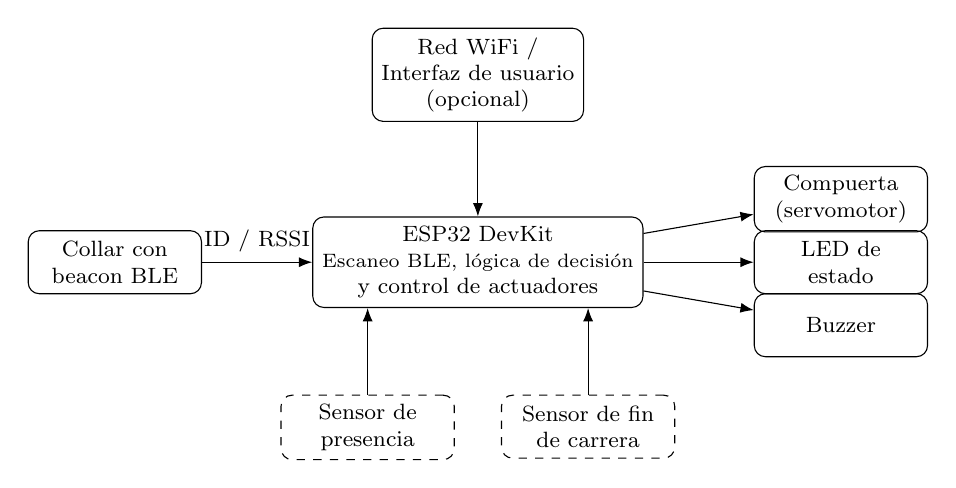
\begin{tikzpicture}[
        font=\footnotesize,
        node distance=0.9cm and 1.4cm,
        block/.style={draw, rounded corners, align=center, minimum width=2.6cm, minimum height=0.9cm},
        smallblock/.style={draw, rounded corners, align=center, minimum width=2.2cm, minimum height=0.8cm},
        sensor/.style={draw, dashed, rounded corners, align=center, minimum width=2.2cm, minimum height=0.8cm},
        line/.style={-Latex}
    ]

    % COLLAR BLE 
    \node[smallblock] (collar) {Collar con\\ beacon BLE};

    % ESP32 
    \node[block, right=of collar] (esp32) {ESP32 DevKit\\
        \scriptsize Escaneo BLE, lógica de decisión\\ y control de actuadores};

    % ACTUADORES 
    \node[smallblock, right=of esp32, yshift=0.8cm] (servo) {Compuerta\\ (servomotor)};
    \node[smallblock, right=of esp32] (led) {LED de\\ estado};
    \node[smallblock, right=of esp32, yshift=-0.8cm] (buzzer) {Buzzer};

    % SENSORES 
    \node[sensor, below=1.1cm of esp32, xshift=-1.4cm] (presencia) {Sensor de\\ presencia};
    \node[sensor, below=1.1cm of esp32, xshift=1.4cm] (limit) {Sensor de fin\\ de carrera};

    % WIFI / INTERFAZ 
    \node[block, above=1.2cm of esp32] (wifi) {Red WiFi /\\ Interfaz de usuario\\ (opcional)};

    % CONEXIONES PRINCIPALES
    \draw[line] (collar) -- node[above]{ID / RSSI} (esp32);

    % Salidas a actuadores
    \draw[line] (esp32) -- (servo);
    \draw[line] (esp32) -- (led);
    \draw[line] (esp32) -- (buzzer);

    % Entradas de sensores
    \draw[line] (presencia.north) -- (esp32.south -| presencia.north);
    \draw[line] (limit.north) -- (esp32.south -| limit.north);

    % Conexión WiFi / interfaz
    \draw[line] (wifi.south) -- (esp32.north);

    \end{tikzpicture}%
    }
    \caption{Diagrama de bloques del sistema propuesto para el arenero inteligente con acceso selectivo.}
    \label{fig:diagrama_bloques}
\end{figure}

\section{Objetivos y Alcances}

\subsection{Objetivo General}

Diseñar e implementar un prototipo de arenero inteligente con acceso selectivo que, mediante un collar basado en Bluetooth Low Energy (BLE) y un microcontrolador ESP32, permita el ingreso únicamente de un gato autorizado, controlando de manera segura la apertura y cierre de una compuerta.

\subsection{Objetivos Específicos}

\begin{itemize}
    \item Analizar y comparar tecnologías de identificación inalámbrica, con énfasis en BLE y RFID, para justificar la selección de BLE como solución adecuada en términos de coste, consumo y facilidad de integración con el ESP32.
    \item Diseñar el collar con beacon BLE para el gato autorizado, considerando peso, autonomía y fijación, de modo que resulte cómodo y funcional en un entorno doméstico.
    \item Desarrollar el firmware del ESP32 para:
    \begin{itemize}
        \item Escanear dispositivos BLE cercanos y filtrar el identificador correspondiente al collar autorizado.
        \item Estimar la proximidad mediante RSSI y definir umbrales para la activación de la compuerta.
        \item Gestionar el control del servomotor, del buzzer y del LED de estado, así como la lectura de los sensores de presencia y fin de carrera.
    \end{itemize}
    \item Integrar los componentes electrónicos con la estructura física del arenero, implementando un mecanismo de compuerta que se abra únicamente cuando el gato autorizado se aproxima y se cierre de forma segura una vez completado el ingreso/salida.
    \item Realizar pruebas funcionales en un entorno controlado, evaluando la tasa de detección correcta del gato autorizado, la respuesta del sistema ante otros dispositivos BLE y el comportamiento mecánico de la compuerta.
    \item Documentar la arquitectura resultante, las decisiones de diseño y las limitaciones observadas, de manera que el prototipo pueda ser replicado o extendido en trabajos futuros.
\end{itemize}

\subsection{Alcances y Limitaciones}

El proyecto se enmarca en el desarrollo de un prototipo funcional de tipo prueba de concepto. Los alcances y limitaciones se definen de la siguiente manera:

\subsubsection*{Alcances}

\begin{itemize}
    \item Implementar un arenero con una única compuerta motorizada controlada por un ESP32, capaz de abrirse sólo ante la detección del identificador BLE del gato autorizado.
    \item Utilizar un único collar con beacon BLE para un gato específico, centrando las pruebas en el acceso selectivo de ese individuo.
    \item Incluir sensores básicos de seguridad (presencia y fin de carrera) para evitar cierres peligrosos y detectar estados anómalos de la compuerta.
    \item Implementar una interfaz mínima de monitoreo (por ejemplo, mensajes por puerto serie o registro simple vía WiFi) que permita observar eventos de acceso y estados del sistema durante las pruebas.
\end{itemize}

\subsubsection*{Limitaciones}

\begin{itemize}
    \item El prototipo no contempla, en esta fase, funciones avanzadas de autolimpieza del arenero (como tamizado automático de arena), más allá de la posibilidad de integrarlas en trabajos posteriores.
    \item No se implementará un sistema completo de gestión multi-gato con múltiples collares y reglas complejas; el enfoque se limita a un único gato autorizado y al bloqueo del acceso para otros individuos.
    \item La solución no está pensada para producción comercial ni cuenta con certificaciones formales de seguridad eléctrica o de compatibilidad electromagnética.
    \item Las pruebas se realizarán en un entorno controlado y con un número reducido de escenarios; no se evalúan aspectos de robustez a largo plazo, resistencia a condiciones extremas o comportamiento en hogares con muchos dispositivos inalámbricos simultáneos.
\end{itemize}

Estos alcances y limitaciones permiten acotar el proyecto a un objetivo realista y abordable dentro del tiempo disponible, manteniendo al mismo tiempo una base tecnológica sólida sobre la cual se pueden proponer mejoras y extensiones en futuras iteraciones.

\ifCLASSOPTIONcaptionsoff
  \newpage
\fi

\begin{thebibliography}{9}

\bibitem{walker2024ble}
A.~M. Walker, N.~N. Jonsson, A.~Waterhouse \emph{et al.},
``Development of a novel Bluetooth Low Energy device for proximity and location monitoring in grazing sheep,''
\emph{Animal}, vol.~18, p.~101276, 2024.
doi: \url{https://doi.org/10.1016/j.animal.2024.101276}.

\bibitem{fonseca2023wearable}
L.~Fonseca, D.~Corujo, W.~Xavier, and P.~Gonçalves,
``On the Development of a Wearable Animal Monitor,''
\emph{Animals}, vol.~13, no.~1, p.~120, 2023.
doi: \url{https://doi.org/10.3390/ani13010120}.

\bibitem{wild2023selective}
S.~Wild, G.~Alarc\'on-Nieto, M.~Chimento, and L.~M. Aplin,
``Manipulating actions: A selective two-option device for cognitive experiments in wild animals,''
\emph{Journal of Animal Ecology}, vol.~92, no.~8, pp.~1509--1519, 2023.
doi: \url{https://doi.org/10.1111/1365-2656.13756}.

\bibitem{farine2024blebeacons}
D.~R. Farine, J.~Penndorf, S.~Bolcato, B.~Nyaguthii, and L.~M. Aplin,
``Low-cost animal tracking using Bluetooth low energy beacons on a crowd-sourced network,''
\emph{Methods in Ecology and Evolution}, vol.~15, no.~12, pp.~2247--2261, 2024.
doi: \url{https://doi.org/10.1111/2041-210X.14433}.

\bibitem{gendy2023blevsrfid}
M.~E.~G. Gendy, P.~Tham, F.~Harrison, and M.~R. Yuce,
``Comparing Efficiency and Performance of IoT BLE and RFID-Based Systems for Achieving Contact Tracing to Monitor Infection Spread among Hospital and Office Staff,''
\emph{Sensors}, vol.~23, no.~3, p.~1397, 2023.
doi: \url{https://doi.org/10.3390/s23031397}.

\bibitem{brian2023petfeeder}
J.~Brianbojoyou, A.~Ashivin, V.~Abilash, and V.~M. Bhaskaran,
``Automated Pet Feeder with RFID Technology using Design Thinking Approach,''
\emph{International Journal for Research in Applied Science \& Engineering Technology (IJRASET)}, vol.~11, no.~11, pp.~1090--1096, 2023.
doi: \url{https://doi.org/10.22214/ijraset.2023.56668}.

\bibitem{zainal2023litterbox}
M.~H. Zainal and K.~L. Chua,
``Development of Automatic Litter Box Using ESP32,''
\emph{Evolution in Electrical and Electronic Engineering (EEEE)},
vol.~4, no.~2, pp.~529--536, Oct.~2023, Accessed: Nov.~14, 2025.
[Online]. Available:
\url{https://publisher.uthm.edu.my/periodicals/index.php/eeee/article/view/13195}


\bibitem{seema2025littertray}
M.~Seema, M.~Prince, J.~P. P.~M., and A.~Sumithra,
``An IoT-Enabled System for Monitoring and Alerting Cat Litter Tray Cleaning Based on Fill-Level Detection,''
\emph{International Journal of Environmental Sciences}, vol.~11, no.~22s, pp.~5107--5114, 2025.
doi: \url{https://doi.org/10.64252/jezsxz36}.

\end{thebibliography}

\end{document}